\documentclass[tufte-handout]{standalone}
\usepackage{mathpazo} % Sets Palatino as the main font
\usepackage{tikz}
\usetikzlibrary{3d, angles, quotes, calc, backgrounds}
\usetikzlibrary{decorations.markings}

% my colors
\definecolor{darkslategray}{rgb}{0.18, 0.31, 0.31}
\definecolor{myorange}{rgb}{0.89804, 0.55686, 0.19608}

\begin{document}

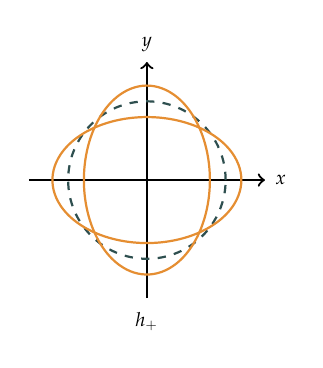
\begin{tikzpicture}
% Define styles
\tikzset{circle grid/.style={darkslategray, thick, dashed}}

% Parameters
\def\stretch{0.2} % Amplitude of the stretch

% h+ Polarization
\begin{scope}[shift={(-5,0)}] % Shift left
  % Draw axes
  \draw[->, thick] (-1.5,0) -- (1.5,0) node[right] {\scriptsize $x$};
  \draw[->, thick] (0,-1.5) -- (0,1.5) node[above] {\scriptsize $y$};
  
  % Draw original circle
  \draw[circle grid] (0,0) circle (1);

  % Draw deformed ellipse (h+)
  \draw[thick, myorange] plot[domain=0:360, smooth, samples=100] 
    ({cos(\x) * (1 + \stretch * cos(2))}, {sin(\x) * (1 - \stretch * cos(2))});
  \draw[thick, myorange] plot[domain=0:360, smooth, samples=100] 
    ({cos(\x) * (1 - \stretch * cos(2))}, {sin(\x) * (1 + \stretch * cos(2))});
  % Title
  \node at (0,-1.8) {\scriptsize $h_+$};
\end{scope}

\end{tikzpicture}

\end{document}

